\documentclass[12pt]{article}
\usepackage{fancyhdr}
\usepackage[T1]{fontenc}
\usepackage{graphicx}
\usepackage{listings}
\pagestyle{fancy}
\rhead{Vince Lehman\\UID: 00473930\\COMP 4262\\Project\\12/2/14}
\renewcommand{\headrulewidth}{0pt}
\begin{document}
\ \\
\section{Objective and Summary}

\textbf{Smartdel} is a Linux command line script designed to supplement the unforgiving \texttt{rm} command. It is very
common for a user, whether inexperienced or command line pro, to unintentionally delete an important file. Smartdel
aims to give the user an experience similar to the recycling bin option in most operating system GUIs. Recycling bins give
the user the option of removing a file from a directory and keeping their workspace uncluttered while at the same time,
allow the user to restore a file that has been previously removed. This implementation allows a user to delete a file, or multiple
files using wildcards, and at any later time, restore the original file for the user to continue to use as if the file had never been
deleted.

\section{Overview and Detailed Design}

Smartdel was designed with the intent of being as modular and simply designed as possible. To store deleted files, Smartdel
uses a directory created in the user's home directory. When the included \texttt{install.sh} script is run, the directory
\texttt{.recycle} is created in the user's home directory and the \texttt{smartdel} script is installed in \texttt{/usr/local/bin}.
When a file is deleted, the \texttt{mv} command is used to remove the file from the current directory and store it in the
recycling directory. When a file is restored, the file is moved from the recycling directory to the user's current directory.

An interesting design consideration was the use of wildcards when deleting and restoring files. When deleting files, Bash
automatically expands the regular expression and passes the matching files as arguments to the script. Thus, the script
can simply iterate over the files provided as arguments and move them to the recycling directory. When restoring files,
it is undesirable to have Bash expand the regular expression since the intent is not to match files in the current directory
but instead to match files in the recycling directory. Therefore, wildcard regular expressions must be enclosed in double
quotes when restoring files. The pattern passed as an argument is appended to the recycling directory and used to
iterate over the matching files; these matching
\newpage
\thispagestyle{empty}
files are then moved to the user's current directory.

Included below is a flow chart detailing the above logic for deleting and restoring files:

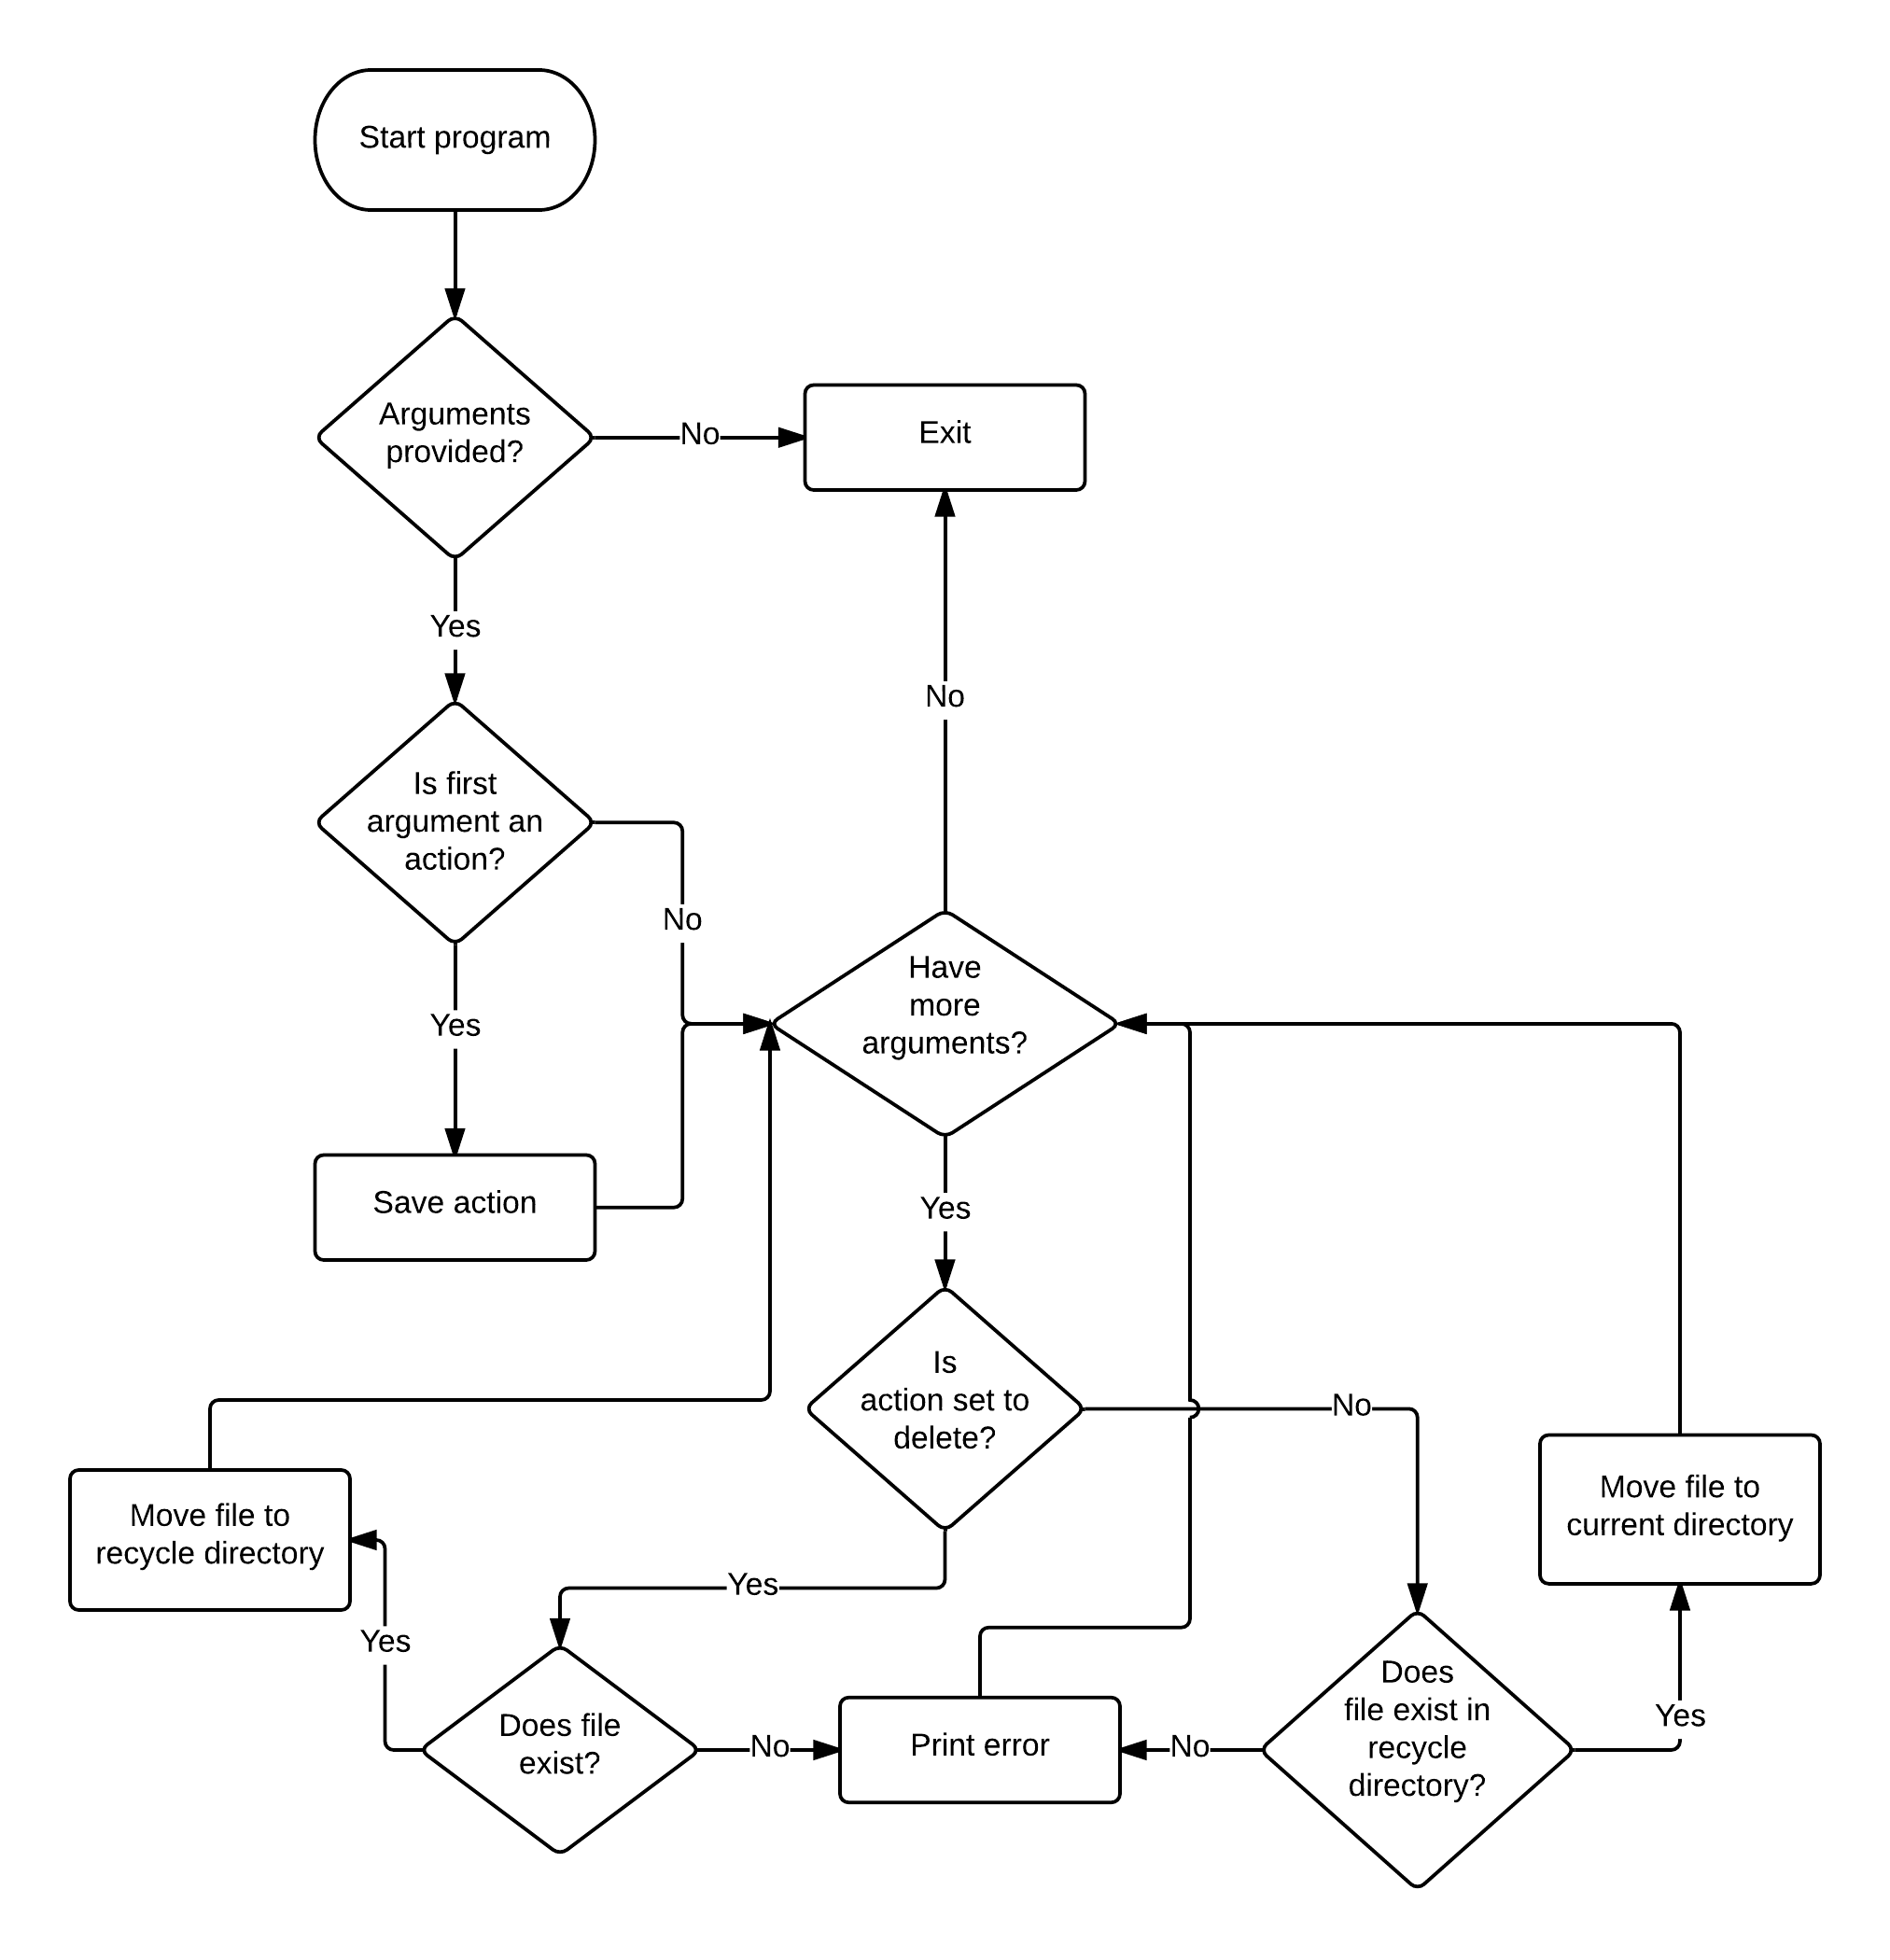
\includegraphics[width=\linewidth]{img/flow-chart}

\section{Testing Procedures and Results}

Smartdel was designed initially to simply pass tests with the examples provided in the project description. As additional features
were added, more robust test cases were run. For example, many tests were run for boundary cases and incorrect usage such as
no files provided as arguments, out of order arguments, and restoring and deleting nonexistent files. These tests helped in catching
errors that were not originally handled by the program and helped to influence the design of deleting and restoring functions.
 
\section{Discussions and Extra Credit Efforts}

Some potential cases are not handled by this implementation of Smartdel, but the issues were considered and there are many possible
solutions to the problems. In the case where deleted files have the same name, the current implementation will simply overwrite the
previous file with the same name. Instead, a file could be used as a sort of database to store a file name with its original directory. When
the user restores a file, the script can check the user's current directory and find the file that matches the name and current directory.

In the case where a file is restored to a directory where a file with that name already exists, the file could be restored with "smartdel"
appended to the original filename. If a file with that name has been previously restored by Smartdel, the program can append a number
greater than the previous number (i.e., restore file "example.txt" as "example.txt-smartdel", subsequent restorations would append
numbers "example.txt-smartdel-2", "example.txt-smartdel-3", etc).
\section{Conclusions}
\thispagestyle{empty}
This implementation of Smartdel was able to accomplish the goals set forth by the course description and the goals established for
software design. The code implements the necessary functionality while using a straightforward and simple design. The current design
does not address potentially critical issues of concern, but the issues could be fixed in the current design using the above proposed
solutions.

\end{document}